\documentclass[notheorems, 10pt]{beamer}
\usepackage[absolute , overlay]{textpos}
\usepackage[italian]{babel}
\usepackage{multicol}
\usepackage{animate}




%%%%%%%%%%%%%%%%%%%%%%%%%%%%%
%%%%% TEMA
%%%%%%%%%%%%%%%%%%%%%%%%%%%%%%
\makeatletter
  \def\beamer@calltheme#1#2#3{%\def\beamer@themelist{#2}
    \@for\beamer@themename:=\beamer@themelist\do
    {\input{Beamer/#3\beamer@themename.sty}}}

\usetheme[math]{beunitn}




%%%%%%%%%%%%%%%%%%%%%%%
%%%%% TEOREMI: FORMATTAZIONE
%%%%%%%%%%%%%%%%%%%%%%%
\theoremstyle{definition}
\newtheorem{definition}{Definizione}



%%%%%%%%%%%%%%%%%%%%%%%%%%%%%%%
%%%%%%%% METADATA
%%%%%%%%%%%%%%%%%%%%%%%%%%%%%%%
\title{Processi gaussiani e apprendimento supervisionato: applicazione al modello Windkessel}
\date{}
\author{Stefano Costa \\ prof. Lucas Omar Müller}
\titlegraphic{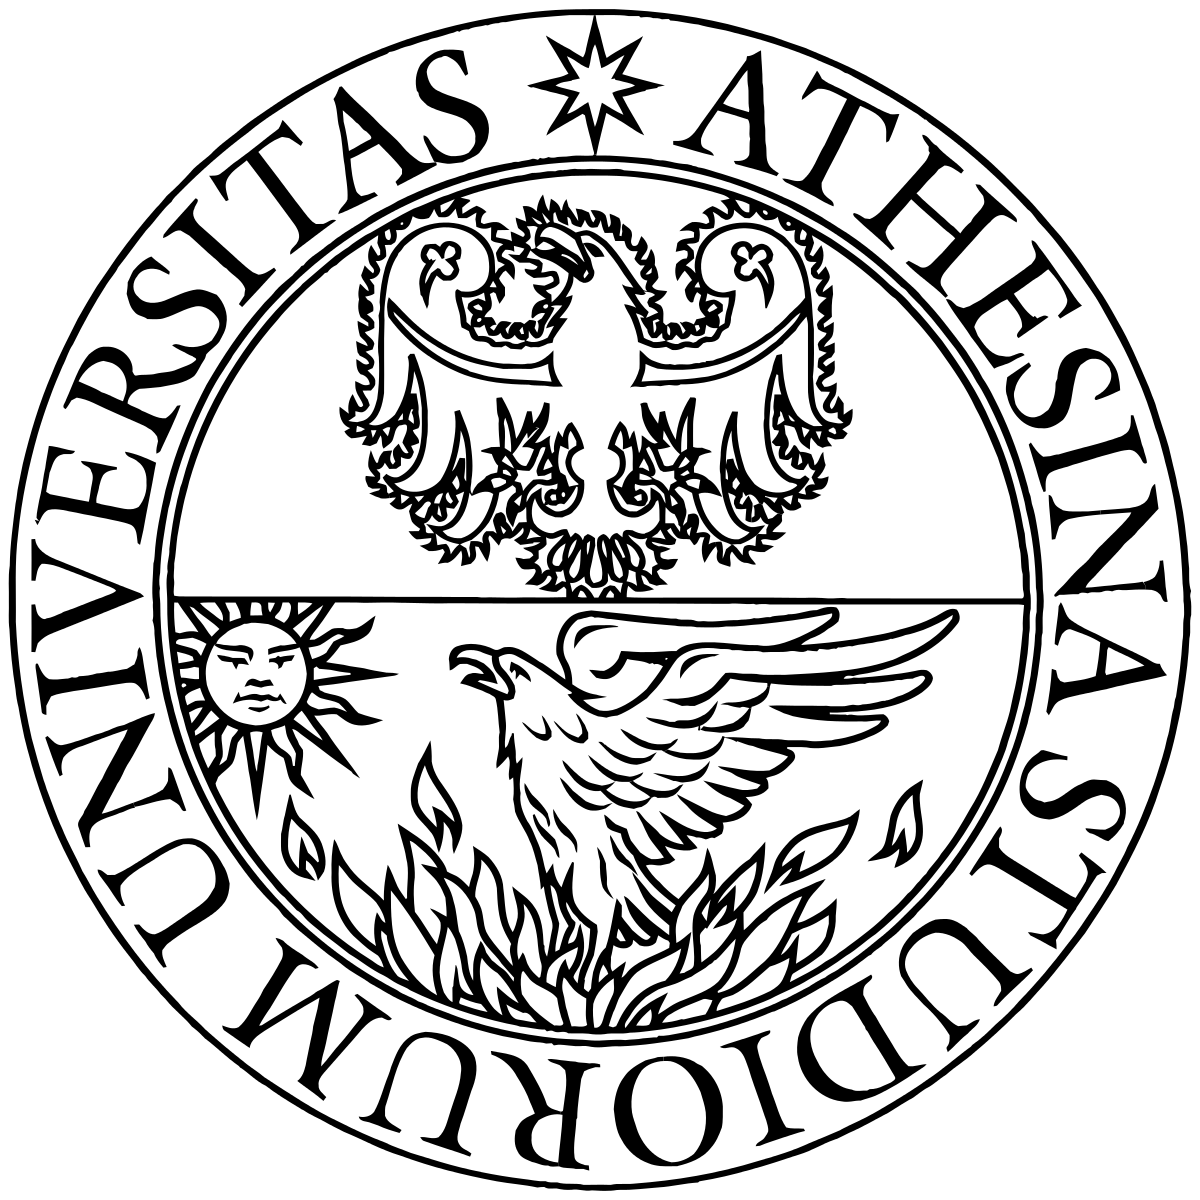
\includegraphics[width=0.2\textwidth]{logo}}




%%%%%%%%%%%%%%%%%%%%%%%%%%%%%%%%%%
\begin{document}


\begin{frame}{}
    \titlepage
\end{frame}

\begin{frame}{Indice}
    \tableofcontents
\end{frame}


%%%%%%%%%%%%%%%%%%%%
%%%%%%%%% DISTRIBUZIONE GAUSSIANA
%%%%%%%%%%%%%%%%%%%%
\section{Correlazione}




\begin{frame}{Correlazione: gaussiane bivariate}
    \vspace{-0.7cm}
    \only<1>{
    \begin{columns}
        \begin{column}{0.65\textwidth}
            \begin{center}
                 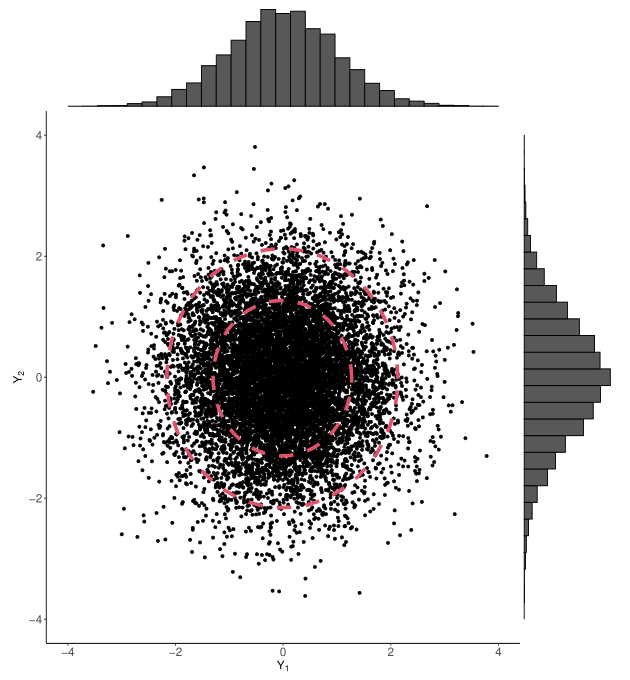
\includegraphics[width=1\textwidth]{images/Gaussiane/VettoreBivariatoIndipendenza.png}
            \end{center}
        \end{column}
        \begin{column}{0.35\textwidth}  
            \[
             \bm{\mu} = \begin{pmatrix}0\\0\end{pmatrix}  
            \]
            \[
            \mathbf{\Sigma}=\begin{pmatrix}1&0\\0&1\end{pmatrix}
            \]
            \[
            \rho_{X,Y}=0
            \]
        \end{column}
    \end{columns}
    }
    
    \only<2>{
    \begin{columns}
        \begin{column}{0.65\textwidth}
            \begin{center}
                 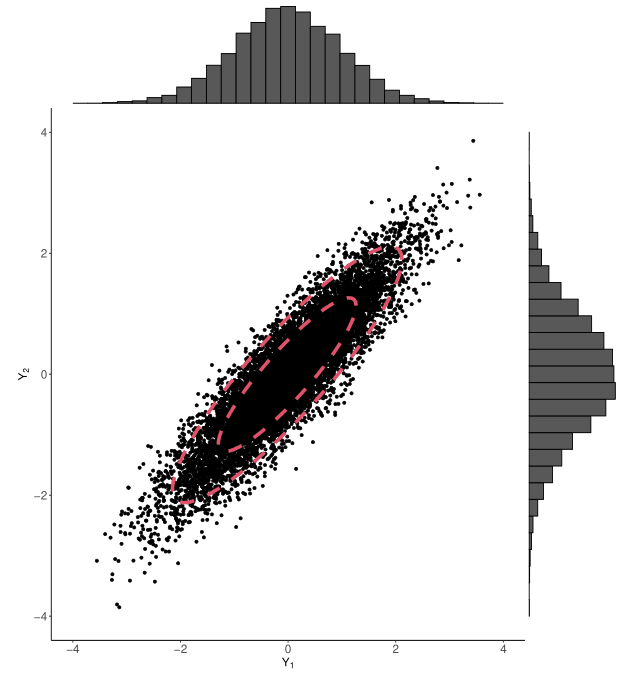
\includegraphics[width=1\textwidth]{images/Gaussiane/VettoreBivariatoIndipendenza2.png}
            \end{center}
        \end{column}
        \begin{column}{0.35\textwidth}  
            \[
             \bm{\mu} = \begin{pmatrix}0\\0\end{pmatrix}  
            \]
            \[
            \mathbf{\Sigma}=\begin{pmatrix}1&0.9\\0.9&1\end{pmatrix}
            \]
            \[
            \rho_{X,Y}=0.9
            \]
        \end{column}
    \end{columns}
    }
    
    \only<3>{
    \begin{columns}
        \begin{column}{0.65\textwidth}
            \begin{center}
                 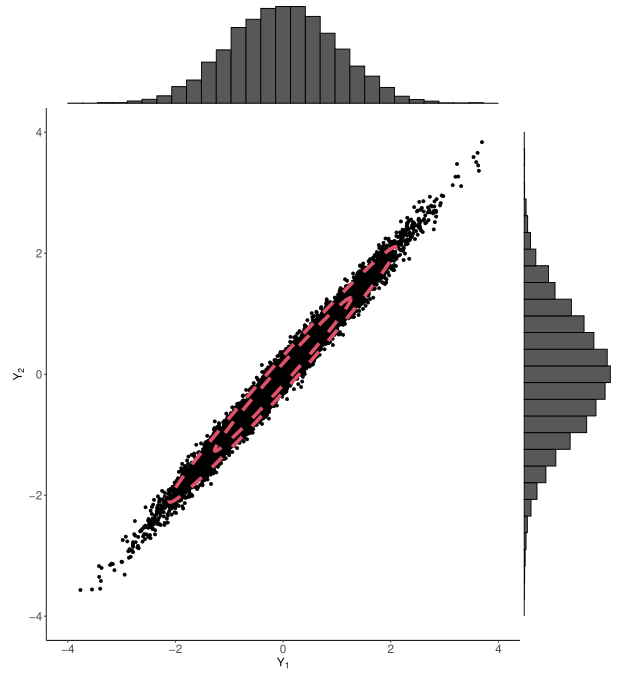
\includegraphics[width=1\textwidth]{images/Gaussiane/VettoreBivariatoIndipendenza3.png}
            \end{center}
        \end{column}
        \begin{column}{0.35\textwidth}  
            \[
             \bm{\mu} = \begin{pmatrix}0\\0\end{pmatrix}  
            \]
            \[
            \mathbf{\Sigma}=\begin{pmatrix}1&0.99\\0.99&1\end{pmatrix}
            \]
            \[
            \rho_{X,Y}=0.99
            \]
        \end{column}
    \end{columns}
    }

\end{frame}

\begin{frame}{Correlazione: gaussiane bivariate}
    \center
    \vspace{-0.7cm}
    \only<1>{
        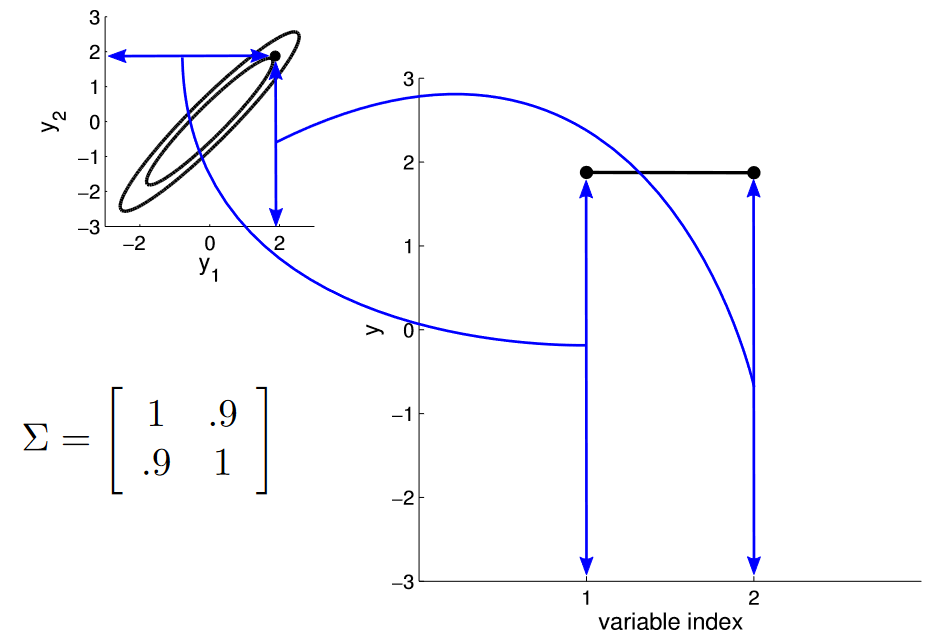
\includegraphics[width=0.8\textwidth]{images/Beamer/Interpretazione visiva.PNG}
    }
    %%%%%%%%%%%%%%%%%
    %%% p=0.9
    %%%%%%%%%%%%%%%%%
    \only<2>{
        \animategraphics[autoplay , loop,width=0.8\textwidth]{4}{./images/Beamer/Prima correlazione/}{1}{20}
    }
    %%%%%%%%%%%%%%%%%
    %%% Person per ogni coppia X,Y è ogni elemento sopra la diagonale
    %%%%%%%%%%%%%%%%%
    \only<3>{
        \animategraphics[autoplay , loop,width=0.8\textwidth]{4}{./images/Beamer/Seconda correlazione/}{1}{20}
    }
\end{frame}

\begin{frame}{Effetto Windkessel}

    \only<1>{
        \begin{definition}[Capacitanza o compliance]
            È la capacità di un organo cavo di distendersi e aumentare di volume con l'aumento della pressione. La compliance $C$ di un vaso sanguigno è direttamente proporzionale all'elasticità delle sue pareti e costituisce una misura dei rapporti tra le variazioni di pressione e le variazioni di volume. 
            \[
            C=\frac{\Delta V}{\Delta P} \quad \left(\frac{mL}{mmHg}\right)
            \]
            $\Delta V$ variazione di volume\\
            $\Delta P$ variazione di pressione (differenza tra pressione intravasale e esterna)
        \end{definition}
    }

    \only<2>{
        \center
        \vspace{-0.7cm}
        \begin{columns}
            \begin{column}{0.5\textwidth}
                \begin{center}
                    \animategraphics[autoplay, loop,width=\textwidth]{20}{./images/Beamer/no windkessel/}{1}{31}
                \end{center}
            \end{column}
            \begin{column}{0.5\textwidth}  
                \animategraphics[autoplay, loop,width=\textwidth]{15}{./images/Beamer/windkessel/}{1}{50}
            \end{column}
        \end{columns}
    }
\end{frame}



\begin{frame}{Fonti immagini}
    %\cite{wilkinson_introduction_2020}
    ...
\end{frame}





\end{document}